\documentclass[11pt,a4paper]{article}
\usepackage[utf8]{inputenc}
\usepackage{amsmath}
\usepackage[czech]{babel}
\usepackage{amsfonts}
\usepackage{amssymb}
\usepackage{graphicx}
\usepackage{subcaption}
\usepackage{a4wide}
\usepackage{siunitx}
\usepackage{booktabs}
\usepackage{empheq}
\usepackage[most]{tcolorbox}
\newtcbox{\mymath}[1][]{%
	nobeforeafter, math upper, tcbox raise base,
	enhanced, colframe=blue!30!black,
	colback=blue!30, boxrule=1pt,
	#1}
\usepackage[figurename=Obr., tablename=Tab.]{caption}
\sisetup{output-decimal-marker = {,}}
\usepackage[version=4]{mhchem}
\usepackage[colorlinks=true,urlcolor=black,citecolor=blue]{hyperref}
%\usepackage{cleveref}
\author{Michal Šesták}
\title{Čip v sudu s radonovou atmosférou}
\begin{document}
\maketitle	
\tableofcontents
\section{Úvod}
Účelem tohoto experimentu je zkoumání vlivu kosmického záření na chybovost integrovaného obvodu. Kosmické záření je simulováno radonovou atmosférou v plechovém uzemněném sudu válcové geometrie, v jehož středu je čip umístěn. Radonová atmosféra je vytvořena injekcí definované koncentrace radonu do sudu v daný počáteční čas. Kolem čipu jsou umístěny TLD detektory, kterými měříme dávku absorbovanou v čipu. Dále se měří počet chyb zaznamenaných v různých segmentech čipu, např v ADC nebo v paměti. Snahou je zjistit, zdali existuje nějaká závislost počtu chyb v čipu na velikosti absorbované dávky.

Problémem je, že zatímco $\beta$ a $\gamma$ záření je TLD detektory měřeno spolehlivě, u $\alpha$ tomu tak není. Proto se přistoupilo k pokusu o výpočet dávky z jednotlivých složek záření ($\alpha, \beta, \gamma$) pomocí teoretických poznatků. 

Ještě předtím však bylo potřeba ověřit, že radon difunduje do zkoumaného čipu přes vrstvičku materiálu, která ho obklopuje, dostatečně rychle vzhledem k jeho radioaktivní přeměně. Pokud by difundoval mnohem pomaleji než se přeměňuje, pak by dávka (hlavně její část pocházející od alf) byla nižší než v případě, kdy bychom uvažovali stejnou koncentraci radonu v čipu jako v okolním prostředí sudu. Proto byl výpočet dávky rozdělen do dvou úloh.
\section{Úlohy}
\begin{enumerate}
	\item Ověření, zdali radon difunduje k čipu přes vrstvičku materiálu pouzdra dostatečně rychle vzhledem k radioaktivní přeměně radonu v sudu.
	\item Výpočet dávky absorbované v čipu. Určují se jednotlivě příspěvky od záření $\alpha, \beta, \gamma$.
\end{enumerate}
\section{Difúze radonu do čipu skrze pouzdro}
\subsection{Popis difúzního šíření}
Průběh šíření radonu difúzí v čase v daném materiálu popsaném difúzním součinitelem $D$ se řídí druhým Fickovým zákonem
\begin{equation}
\frac{\partial c}{\partial t}=D\cdot \text{div}(c)-\lambda c\,,\label{eq:fickuvLawObecne}
\end{equation}
kde $c=c(t;x,z,y)$ je koncentrace radonu v bodě $(x,y,z)$ v čase $t$, $\lambda$ je přeměnová konstanta radonu; $[c]=\si{Bq/m^3}$; $[D]=\si{m^2s^{-1}}$. 

\subsection{Součinitel difúze a rozměry pouzdra}
Vzhledem k tomu, že známe pouze prvkové složení pouzdra a nevíme, z jakého materiálu je vyrobeno, tak byl uvažován difúzní součinitel o hodnotě
\begin{equation}
D=\SI[parse-numbers = false]{3\cdot 10^{-7}}{m^2s^{-1}}\,,
\end{equation}
což by měla být hodnota obvyklá pro pevné látky (zdroj?\footnote{zkusit najít a doplnit}). Čip je rozměrově kvádr o šířce a délce cca 7 mm a tloušťce 0,15 mm. Pouzdro ho obepíná, na bočních stranách čipu je 6,5 až 7 mm materiálu pouzdra, na horní a dolní ploše čipu je ho 0,69 mm. 

\subsection{Numerické řešení difúzní rovnice}\label{pol:aproximace}
Řešení rovnice \eqref{eq:fickuvLawObecne} v kartézských souřadnicích při daných rozměrech pouzdra by bylo zbytečně náročné, a proto se přistoupilo k aproximaci čipu koulí o poloměru $R_1$ a pouzdra kulovou slupkou o poloměru $R_2$ a tloušťce $d$. Pak lze rovnici \eqref{eq:fickuvLawObecne} převést do sférických souřadnic $(r, \varphi, \phi)$ s počátkem ve středu aproximujících útvarů:
\begin{equation}
\frac{\partial c}{\partial t}=D\left(\frac{\partial^2c}{\partial r^2}+\frac{2}{r}\frac{\partial c}{\partial r}\right)-\lambda c\,,\label{eq:fick}
\end{equation}
kde navíc díky homogennosti koncentrace radonu v okolí pouzdra uvažujeme izotropní šíření, tj. nezávislé na souřadnicích $\varphi$ a $\phi$, a proto $c=c(t,r)$. V prvním přiblížení byly aproximující parametry položeny hodnotám
\begin{align}
	R_1&=\SI{5}{cm}\,,\\
	R_2&=\SI{10}{cm}\,,\\
	d=R_2-R_1&=\SI{5}{cm}\,,
\end{align}
v případě potřeby by byly zmenšeny. Rovnice \eqref{eq:fick} byla řešena jen uvnitř pouzdra. 
\subsubsection{Počáteční a okrajové podmínky}
Byly řešeny dva případy:
\begin{enumerate}
	\item \textbf{Injektáž radonu:} v okolí čipu je konstantní koncentrace radonu $c_0$ a uvnitř čipu a pouzdra je v počátečním čase nulová koncentrace, tj.:
	\begin{itemize}
		\item počáteční podmínka je $c(0,r)=c_u(0)=0$ pro $r\in(R_1, R_2)$, kde $c_u(t)$ je koncentrace radonu v kouli aproximující čip v blízkosti pouzdra,
		\item okrajová podmínka na rozhraní pouzdra a okolního prostředí (dále jen vnější okrajová podmínka) je $c(t,R_2)=c_0$ pro $t\in[0,T]$, kde $T$ čas, do kterého chceme rovnici řešit,
		\item okrajová podmínka na rozhraní pouzdra a čipu (dále jen vnitřní okrajová podmínka) bude uvedena později.
	\end{itemize}
	 
	\item \textbf{Vypumpování radonu:} v okolí čipu je nulová koncentrace radonu a uvnitř čipu a pouzdra je koncentrace tentokrát v počátečním čase $c_0$, tedy:
	\begin{itemize}
		\item počáteční podmínka je $c(0,r)=c_u(0)=c_0$ pro $r\in[R_1, R_2]$,
		\item vnější okrajová podmínka je $c(t,R_2)=0$ pro $t\in[0,T]$,
		\item vnitřní okrajová podmínka bude uvedena později.
	\end{itemize} 
\end{enumerate}
První případ představuje injektáž radonu do sudu s čipem, druhý pak vypumpování radonu ven ze sudu. Vnitřní okrajová podmínka vypadá následovně:
\begin{equation}
	D\frac{\partial c(t,R_1)}{\partial r}=h\cdot(c(t,R_1)-c_u(t))\,,\label{eq:vnitrniOkrPodm}
\end{equation}
kde $h$ je tzv. přestupní koeficient vyjadřující schopnost přestupu radonu z pouzdra do čipu (nebo naopak), $[h]=\si{m\cdot s^{-1}}$. Jeho určení je velmi problematické a v podstatě nebyla provedena žádná systematická měření jeho hodnot pro rozhraní různých materiálů. Autoři článku~\cite{jiranek1} odhadují jeho hodnotu pro nezměřená rozhraní na
\begin{equation}
	h=\SI{0,1}{m\cdot s^{-1}}\,,
\end{equation}
tato hodnota byla uvažována i v našich výpočtech.

Koncentrace uvnitř čipu $c_u(t+\Delta t)$ se určí ze známé koncentrace v předchozím bodě časové sítě $c_u(t)$ pomocí vztahů
\begin{align}
	E(t)&=h\cdot(c(t,R_1)-c_u(t))\,,\label{eq:exhalace}\\
	c_u(t+\Delta t)&=c_u(t)\cdot \mathrm{e}^{-\lambda\Delta t}+\frac{E(t)\cdot A}{V\cdot \lambda}\cdot \left(1-\mathrm{e}^{-\lambda\Delta t}\right)\,,\nonumber\\
	&=c_u(t)\cdot \mathrm{e}^{-\lambda\Delta t}+\frac{3\cdot E(t)}{R_1\cdot \lambda}\cdot \left(1-\mathrm{e}^{-\lambda\Delta t}\right)\,,\label{eq:vnitrek}
\end{align}
kde $E(t)$ exhalační rychlost z pouzdra do čipu (či naopak) v čase $t$, $[E]=\si{Bq\cdot m^{-2}s^{-1}}$, dále $\Delta t$ je časový krok, $\lambda$ je přeměnová konstanta radonu, $A=4\pi R_1^2$ je vnější plocha koule reprezentující čip a $V=\frac{4}{3}\pi R_1^3$ je objem této koule. Vztahy \eqref{eq:vnitrniOkrPodm}, \eqref{eq:exhalace} a \eqref{eq:vnitrek} byly převzaty z \cite{jiranek1}.

Vnější okrajová podmínka představuje Dirichletovu okrajovou podmínku, vnitřní pak Neumannovu okrajovou podmínku.
\subsubsection{Použitá metoda}
Pro určení prostorového a časového vývoje koncentrace v pouzdře $c(t,r)$ pro $t\in[0, T], r\in[R_1, R_2)$ a časového vývoje koncentrace uvnitř čipu v blízkosti pouzdra $c_u(t)$ pro $t\in[0,T]$ z rovnic \eqref{eq:fick}, \eqref{eq:vnitrniOkrPodm} a \eqref{eq:vnitrek} byla použita Crank-Nicolsonova metoda \cite{numerical_methods, wiki}. 

Z takto určeného vývoje je možné stanovit dobu $T_1$, resp. $T_2$ (pro první a druhý případ), po níž bude radon difundovat přes pouzdro do čipu, dokud nebude v čipu s určitou tolerancí $\varepsilon$ stejná koncentrace radonu jako ve vnějším prostředí. Při výpočtu byla použita tolerance
\begin{equation}
	\varepsilon=0,01\,.
\end{equation}
\subsection{Výsledek}
\begin{figure}[t!]
	\centering
	\begin{subfigure}{.7\textwidth}
		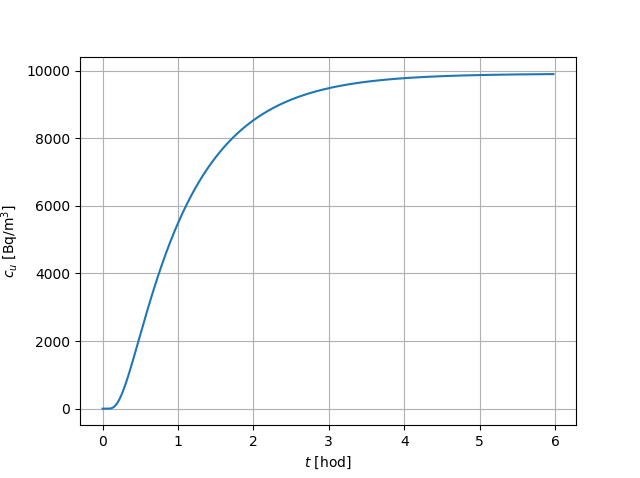
\includegraphics[width=\linewidth]{narust}
		\caption{}
		\label{fig:narust}
	\end{subfigure}
	\begin{subfigure}{.7\textwidth}
		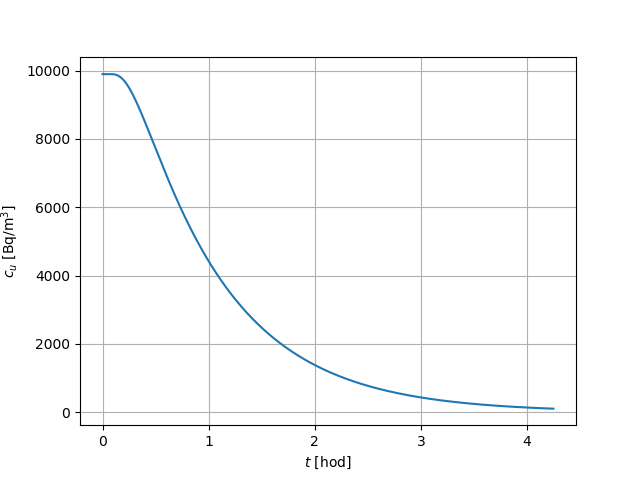
\includegraphics[width=\linewidth]{pokles}
		\caption{}
		\label{fig:pokles}
	\end{subfigure}
\caption{V (a) je vidět časový vývoj koncentrace radonu v čipu v bezprostřední blízkosti pouzdra v prvním uvažovaném případě (injektáž radonu). V (b) je vidět vývoj $c_u$ pro druhý případ (vypumpování radonu ze sudu ven). V tomto případě $c_0=\SI{10}{kBq/m^3}$.}
\label{fig:vyvoj_uvnitr}
\end{figure}
Časový vývoj $c_u$ je pro oba dva případy k nahlédnutí v obr.~\ref{fig:vyvoj_uvnitr}. $T_1$ a $T_2$ vychází pro všechna testovaná $c_0$ stejně:
\begin{align}
	T_1&=\SI{5,98}{hod}\,,\\
	T_2&=\SI{4,25}{hod}\,,\\
	T_1+T_2&=\SI{10,23}{hod}\,,
\end{align}
doba $T_1+T_2$ představuje celkovou dobu trvání obou případů. Byly testovány následující hodnoty $c_0$: $\SI{1}{kBq/m^3}, \SI{10}{kBq/m^3}, \SI{100}{kBq/m^3}, \SI{1}{MBq/m^3}$
\subsection{Diskuze}
Doby $T_1$, $T_2$ a $T_1+T_2$ jsou v porovnání s $T_{1/2}(\ce{^{222}Rn})=\SI{3,82}{dne}$ krátké. Vzhledem k tomu že výpočet proběhl pro mnohem větší rozměry pouzdra než jaké ve skutečnosti jsou, tak můžeme říct, že v čipu je stejná koncentrace radonu jako v sudu po většinu času experimentu. Toto tvrzení ovšem platí pouze za předpokladu, že uvažovaný součinitel difúze skrze pouzdro $D$ není hodně nadhodnocený.
\subsection{Závěr}
Bylo ověřeno, že radon difunduje skrze pouzdro do čipu dostatečně rychle vzhledem k radioaktivní přeměně radonu.
\begin{thebibliography}{Mm99}
	\bibitem{jiranek1} Jiránek M., Fronka A.: New technique for the determination of radon diffusion coefficient in radon-proof membranes. Radiat Prot Dosimetry. 2008;130(1):22-5. doi: 10.1093/rpd/ncn121.
	\bibitem{numerical_methods} Hellevik, L. R.: Numerical Methods for Engineers. Department of Structural Engineering, NTNU. 2018. Citováno 10. 5. 2019. Dostupné z \url{http://folk.ntnu.no/leifh/teaching/tkt4140/._main068.html#ch5:sec6} a \url{http://folk.ntnu.no/leifh/teaching/tkt4140/._main069.html#ex:52}
	\bibitem{wiki} Wikipedia, The Free Encyclopedia: Crank–Nicolson method. Citováno 10. 5. 2019. Dostupné z \url{https://en.wikipedia.org/wiki/Crank%E2%80%93Nicolson_method}
	\end{thebibliography}
\section{Výpočet dávky absorbované v čipu}
I této úloze aproximuje čip a pouzdro koulemi se středy ve stejném bodě a s poloměry $R_1$, resp. $R_2$:
\begin{align}
	R_1&=\SI{3,0}{mm}\,,\\
	R_2&=\SI{3,1}{mm}\,.
\end{align}
Objem a hmotnost čipu jsou označeny jako $V_{cip}$ a $m_{cip}$. Při výpočtu $m_{cip}$ bylo uvažováno, že celý čip je z křemíku:
\begin{align}
	V_{cip}&=\SI{0,0073}{cm^3}\,,\\
	m_{cip}&=\SI{1.7e-05}{kg}\,.
\end{align}

Objem sudu:
\begin{align}
	V_{sud}=\SI{0,19}{m^3}\,.
\end{align}

Je uvažován faktor nerovnováhy $F=0,1$. Objemová aktivita radonu je označena $a$. Do sudu je na začátku experimentu jednorázově injektována počáteční koncentrace radonu $a_0$. Průběh $a$ v sudu se pak řídí exponenciálním rozpadem.
\subsection{Příspěvek od $\alpha$}
V následujících dvou podkapitolách budou určeny energetické příspěvky od $\alpha$ částic vzniklých mimo a uvnitř čipu při dané aktivitě $a$ za jednotkový časový interval. V následující podkapitole proběhne časová integrace těchto příspěvků a následné podělení hmotností pro určení dávky od $\alpha$ částic.
\subsubsection{Energetický příspěvek od $\alpha$, které vznikly mimo čip a pouzdro}
Částice $\alpha$ o dané počáteční energii $T_0$ má v daném prostředí známý maximální dosah $R_{max}$~\cite{astar}. Proto lze okolo čipu uvažovat kouli o poloměru 
$$R_3=R_{max}+R_2\,,$$
v jejímž objemu vzniklé alfa částice mohou dolétnout k pouzdru. Alfa částice emitované mimo tuto kouli budou zastaveny dříve než doletí k pouzdru čipu. Ztrátu energie částice alfa, která vznikla ve vzdálenosti $r\in[R_2, R_3]$ od pouzdra, po projití vrstvy vzduchu o tloušťce $r$ je možné zjistit z tabelovaných hodnot brzdných schopností \cite{astar} a pomocí následujícího jednoduchého algoritmu:
\begin{enumerate}
	\item \emph{Inicializace}:
	\begin{align*}
	x&=0\,,\\
	  dE&=0\,,\\
	   dx&=0,1\,.
	   \end{align*}
	  $x$ je doposud ušlá dráha alfa částice; $dE$ je ztráta energie, která je vypočítávána v každé iteraci; $dx$ je krok, my jej bereme roven jednomu milimetru.
	\item \emph{Iterace}:
	\begin{align}
		x = x+dx\,,
	\end{align}
	kontrola $x<r$,
	\begin{align*}
	dE &= \frac{dE}{dx}(T_i)\cdot dx\,,\\    
	T_{i+1} &= T_i - dE\,,
	\end{align*}  
	kontrola $dE>0$ a $T_{i+1}>0$. 

$\frac{dE}{dx}(T_i)$ je brzdná schopnost alfa částice o energii $T_i$ ve vzduchu. Spojitá závislost $\frac{dE}{dx}$ na $T$ byla získána interpolováním tabelovaných hodnot z~\cite{astar} kubickým splinem.
\item \emph{Ukončení cyklu}:\\
pokud byla porušena jakákoliv kontrola v předchozím bodě, pak je cyklus ukončen a momentální $T$ je energie, která alfa částici zbyla při příchodu k pouzdru.
\end{enumerate}

Předchozí algoritmus je vlastně funkcí vzdálenosti vzniku alfa částice od pouzdra, tj. $r$, označme ji $f_0(r)$. Po přenásobením korekcí na prostorový úhel
\begin{equation*}
k_1=\frac{1}{2}\cdot\left(1-\frac{r}{\sqrt{r^2+R_1^2}}\right)\,,
\end{equation*}
a faktorem zohledňujícím skutečnost, že nás zajímají alfy z celé slupky s vnitřním poloměrem $r$ a vnějším poloměrem $r+\mathrm{dr}$
\begin{equation*}
	k_2=4\pi r^2\,,
\end{equation*}
získáváme funkci $f(r)$, kterou lze zintegrovat od $R_2$ do $R_3$, tj.
\begin{equation}
	I=\int_{R_2}^{R_3}f(r)=\int_{R_2}^{R_3}k_1(r)\cdot k_2(r)\cdot f_0(r)\mathrm{dr}\,. 
\end{equation}
Tato veličina představuje střední hodnotu zbylé energie alfa částice s danou počáteční energií $T_0$ po dojití k pouzdru, která je přenásobená objemem kulové slupky s poloměry $R_2$ a $R_3$, tj. její rozměr je
\begin{equation}
	[I]=\si{MeV\cdot cm^3}\,.
\end{equation}

Po vydělení $I$ objemem  $V=\frac{4}{3}\pi(R_3^3-R_2^3)$ získáváme střední energii alfa částice u vstupu do pouzdra:
\begin{equation}
	\bar{E}=\frac{I}{V}\,.
\end{equation}
Vypočítané hodnoty $I$, $\bar{E}$ a počáteční kinetické energie $T_0$ alfa částic emitovaných radonem a jeho krátkodobě žijících dceřinných produktů jsou v tabulce~\ref{tab:alfa_energie}.
\begin{table}[ht]
	\centering
	\caption{Počáteční energie, $I$ a $	\bar{E}_{pouzdro}$ alfa částic emitovaných radonem a jeho krátkodobě žijícími dceřinnými produkty (RN=radionuklid).}
	\label{tab:alfa_energie}
	%3.1635352 , 4.10481408, 8.36293245
	%0.00836222, 0.00737454, 0.00493332
	\begin{tabular}{llll}
		\toprule
		RN & $T_0$ [MeV] & $I$ [\si{MeV\cdot cm^3}] & $\bar{E}$ [MeV]\\
		\midrule
		\ce{^{222}Rn} &  5,489 &3,164&0,008\\
		\ce{^{218}Po} &  6,002 &4,105&0,007\\
		\ce{^{214}Po} &  7,689 &8,363&0,005\\
		\bottomrule
	\end{tabular}
\end{table}

\paragraph{Energetický příspěvek:}
Energetický příspěvek od $\alpha$ částic vzniklých mimo objem pouzdra a čipu je možné vypočítat z
\begin{align}
E_{vne}&=(\bar{E}_{222} V_{222}+\bar{E}_{218} V_{218} F+\bar{E}_{214} V_{214} F) a\,,\\
	&=(I_{222}+I_{218}F+I_{214}F)a\quad [\si{MeV}]\,,
\end{align}
kde $F$ je faktor nerovnováhy.

\paragraph{Nadhodnocení:} Bohužel tento postup nezahrnuje ztrátu energie v pouzdru, jelikož v databázi~\cite{astar} nelze definovat vlastní materiály. Pro tyto účely je vhodný program SRIM~\cite{srim}, avšak ten mi nebyl doposud nainstalován. Důsledkem je, že je dávka od tohoto příspěvku nadhodnocena.

\subsubsection{Energetický příspěvek od $\alpha$, které vznikly uvnitř čipu a pouzdra}
Energetický příspěvek těchto $\alpha$ jsem odhadl jako jednu polovinu počátečních energií všech $\alpha$ částici vzniklých v objemu čipu, tj.:
\begin{equation}
 E_{vnitrek}=\frac{1}{2}\cdot(5,489+6,002+7,689)\cdot a\cdot V_{cip}\quad[\si{MeV}]\,.
\end{equation} 
Tento odhad lze odůvodnit tím, že $\alpha$ částice mají malý dosah, a proto pokud nejsou emitovány blízko povrchu čipu směrem ven, tak jsou absorbovány uvnitř čipu.
\subsubsection{Celkový příspěvek k dávce}
Příspěvek od $\alpha$ k dávce je roven:
\begin{empheq}[box=\mymath]{equation}
	D_{\alpha}=\frac{1}{m_{cip}}(E_{vne}+E_{uvnitr})\cdot 1,6\times 10^{-13}\frac{1-\exp(-\lambda T)}{\lambda}\,,
\end{empheq}
kde $1,6\times 10^{-13}$ je převodní faktor z MeV na Jouly, $\lambda$ je přeměnová konstanta radonu a $T$ je doba expozice.
\subsection{Příspěvek od $\beta$}
Toto je stále řešeno, vzhledem k charakteru $\beta$ záření je potřeba použít metody Monte Carlo.
\subsection{Příspěvek of $\gamma$}
in progress
\begin{table}[ht]
	\centering
	\caption{}
	\label{tab:gamy}
	\begin{tabular}{lllll}
		\toprule	 
		{} &  E[keV] &      Y &       mu &    muAbs \\
		\midrule
		222Rn  &   511.0 &  0.076 &  0.08712 &  0.02971 \\
		214Pb  &   352.0 &  0.374 &  0.09800 &  0.02968 \\
		214Pb* &   300.0 &  0.270 &  0.10670 &  0.02932 \\
		214Bi  &   609.0 &  0.460 &  0.08055 &  0.02951 \\
		214Bi* &  1180.0 &  0.210 &  0.05687 &  0.02700 \\
		214Bi  &  1764.0 &  0.150 &  0.04800 &  0.02445 \\
		214Bi  &  2204.0 &  0.050 &  0.04447 &  0.02300 \\
		\bottomrule
	\end{tabular}
\end{table}
\subsection{Konkrétní hodnoty}
Vypočítal jsem $D_{\alpha}$ pro $T=\SI{1}{den}$ a pro injektovanou koncentraci $a_0=\SI{1}{kBq\cdot m^{-3}}$:
\begin{align}
	D_{\alpha}=\SI{5.7}{\mu Gy}
\end{align}
\begin{thebibliography}{Mm99}
	\bibitem{astar} National Institute of Standards and Technology: aStar, Stopping-power and Range Tables for Helium Ions. 14. 5. 2019. Dostupné z \url{https://physics.nist.gov/PhysRefData/Star/Text/ASTAR.html}
	\bibitem{srim} Ziegler, J. F.: SRIM - The Stopping and Range of Ions in Matter. 14. 5. 2019. Dostupné z \url{http://srim.org/} 
\end{thebibliography}
\end{document}